\subsection{Glyph: \glyph{Macromolecule}}
\label{sec:macromolecule}

Many biological processes involve macromolecules: biochemical substances that are built up from the covalent linking of pseudo-identical units. Examples of macromolecules include proteins, nucleic acids (RNA, DNA), and polysaccharides (glycogen, cellulose, starch, etc.).  Attempting to define a separate glyph for all of these different molecules would lead to an explosion of symbols in SBGN, so instead, \SBGNERLone defines only one glyph for all macromolecules.  The same glyph is to be used for a protein, a nucleic acid, a complex sugar, and so on.  The exact nature of a particular macromolecule in a diagram is then clarified using its label and decorations, as will become clear below.  (Future levels of SBGN may subclass the \glyph{macromolecule} and introduce different glyphs to differentiate macromolecules.)

\begin{glyphDescription}

\glyphSboTerm SBO:0000245 ! macromolecule 

\glyphContainer A macromolecule is represented by a rectangular container with rounded corners, as illustrated in \fig{macromolecule}.

\glyphLabel A \glyph{macromolecule} is identified by a label placed in an unbordered box containing a string of characters.  The characters can be distributed on several lines to improve readability, although this is not mandatory.  The label box must be attached to the center of the container.  The label may spill outside of the container.

\glyphAux A \glyph{macromolecule} can carry state variables that can add information about its state (\sect{stateVariable}).  The state of a macromolecule is therefore defined as the vector of all its state variable values.  A state variable is represented by an ellipsoid container, with the long axis of the ellipsoid placed on the border of the \glyph{macromolecule}'s container as illustrated in \fig{macromolecule}.  The label of the state variable (which can precise the type of characteristic represented by the state variable, residue type, residue number etc.) is written within the state variable's container.

A \glyph{macromolecule} can also carry one or several \glyph{units of information} (\sect{unitInfo}).  The units of information can characterise a domain, such as a binding site.  Particular \glyph{units of information} are available for describing the material type (\sect{material-types-cv}) and the conceptual type (\sect{conceptual-types-cv}) of a macromolecule.  The center of the bounding box of a \glyph{unit of information} is located on the mid-line of the border of the macromolecule.

\end{glyphDescription}

\begin{figure}[H]
  \centering
  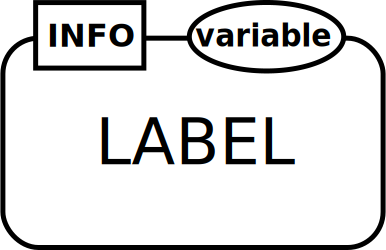
\includegraphics[scale = 0.3]{images/macromolecule}
  \caption{The \ER glyph for \glyph{macromolecule}.}
  \label{fig:macromolecule}
\end{figure}

\normalcolor